\documentclass[conference]{IEEEtran}
\usepackage{ctex}
% CJK 主字体：ctex 默认字集 FandolSong 缺「濙」(U+6FD9) 等字形（PDF 会出现空白/方框），
% 必须用系统华文宋体 STSong（普通 TrueType，xdvipdfmx 可正常子集嵌入）。
% ⚠️ 不要用 Noto Serif SC：本机那版是可变字体 VF，会被 xdvipdfmx 以 Invalid TTC index 拒收。
\setCJKmainfont{STSong}
\usepackage{amsmath}
\usepackage{amssymb}
\usepackage{graphicx}
\usepackage{makecell}
\usepackage{booktabs}
\usepackage{tabulary}

% math_commands.tex —— 全文数学符号与缩略语统一定义（各篇可按需增删，勿改已有通用宏）
\newcommand{\kg}{知识图谱}
\newcommand{\corpus}{语料}
\newcommand{\salience}{叙事热度}
\newcommand{\centre}{中心性}
\newcommand{\Deg}{d}
\newcommand{\Chap}{h}
\newcommand{\Rho}{\rho}
\newcommand{\NP}{\emph{N}}
\newcommand{\bk}[1]{\textbf{#1}}
\newcommand{\cited}[1]{[\cite{#1}]}\newcommand{\pct}[1]{#1\%}
% info 篇正文用到的集合类宏
\newcommand{\Ccal}{\mathcal{C}}
\newcommand{\Dcal}{\mathcal{D}}
\newcommand{\Iec}{\mathcal{I}}
\newcommand{\Igc}{\mathcal{I}_{{gc}}}

% latex_includes.tex —— 只声明图片搜索路径与统一宽度宏
% ⚠️ 禁止在本文件里写 \begin{comment}...\end{comment} 包裹的示例 figure：
%    comment 环境需要 \usepackage{comment}，否则编译直接报
%    "LaTeX Error: Environment comment undefined"（试点篇踩过）。
% 所有 figure 环境一律写在 sections/5_results.tex 内，图题只进 \caption，图内不写标题。
\graphicspath{{figures/}}
\newcommand{\figpath}[1]{figures/#1}


% ⚠️ IEEEtran conference 类不定义 \bibname（那是 book/article 类的宏），
%    加 \renewcommand{\bibname}{...} 会直接编译失败。栏头沿用 venue 原有的英文 References。

\title{谣言、黑名单与告密：帝国的信息战\\[2pt]
\large Denunciation, Blacklist and Rumor: The Information Surveill\\
\large of an Empire}

\author{Anonymous}
\date{}

\begin{document}
\maketitle

%% 中文摘要（200–350 字）：目的 → 数据 → 方法 → 三个结果（带数字）→ 首要限制
\noindent\textbf{摘要（中文）}：本文把一部通俗明代通史（156 章，约 149 万字）抽取出的知识图谱当作
观测对象，检验一个可计算的问题：在没有报纸与电报的时代，通俗史著把帝国的「信息战」写到了什么颗粒度，
又把一个什么样的信息结构交给了图谱。文中先据原书全文逐字核验（0 命中即弃用）建立信息机制词表，
再在 2324 条关系中切出「经信息渠道发动的攻击」，即「政治攻讦」类 193 条（8.3\%）。
三个结果：（1）以全书七部为时间刻度，政治攻讦占该部全部关系的比重从第 1--2 部的 6.4\% 升到第 6--7 部的
16.0\%（$2.48$ 倍），同期对照组「敌对冲突」为 22.7\% 与 22.1\%（$0.98$ 倍，基本不动）；
（2）193 条攻讦中 86.0\% 为跨阵营配对，其端点集与敌对关系仅 86 人重合（Jaccard $0.219$），
端点基尼系数 0.3798，Top-10 只占 $21.0\%$；（3）角色文本含锦衣卫、东厂、西厂的厂卫系 29 人，
平均度数 3.76，与全库 3.78 无差别（$0.99$），只占攻讦端点 $3.6\%$；
而同代这套制度的内廷宦官 51 人平均度数 6.10（$1.61$ 倍）——机构在图谱里隐形，代理人上位。
本文主张：通俗史著把帝国治理写成了一部以人名录展开的程序史。首要限制是关系类别与派系标签
与关系抽取共享同一份语料，攻讦随叙事上升不能排除同源自证；全文所有涉及机构行为的判断
均只落在本书语料内，「信息战」是现代类比而非史实定性。

\noindent\textbf{关键词}：信息战（现代类比）；知识图谱；通俗史学；政治攻讦；
厂卫与内廷宦官；明代叙事结构；数字人文

\vspace{6pt}
%% 英文摘要 150–250 词（aris 硬要求，不许超）
\begin{abstract}
This paper treats a knowledge graph extracted from a best-selling popular history
of the Ming dynasty (156 chapters, about 1.491 million characters) as an object of
observation, and asks a computable question: at what granularity does a popular
history write the {\em information} structures of an empire, and what structure does
it hand to the graph? We first build a vocabulary of information mechanisms by exact
string matching against the original text (any term with zero hits is discarded),
then isolate the attacks that travel through informational channels --- the
``political accusations'' category, $n=193$ of $2{,}324$ relations ($8.3\%$).
Three results follow. First, using the seven parts of the book as a temporal scale,
the share of accusations among all relations in a part rises from $6.4\%$ in parts
1--2 to $16.0\%$ in parts 6--7 (a factor of $2.48$), while the control category
``hostile conflict'' stays flat ($22.7\%$ to $22.1\%$; factor $0.98$). Second, $86.0\%$
of accusation pairs cross faction boundaries, and the endpoint sets of accusations and
hostile conflicts overlap in only $86$ persons (Jaccard $0.219$); the endpoint Gini
coefficient is $0.3798$ and the top ten endpoints hold only $21.0\%$ of all endpoint
occurrences. Third, the $29$ persons whose role text mentions the Brocade Guard or the
East/West Factories have mean degree $3.76$ against a corpus mean of $3.78$ (ratio
$0.99$) and account for only $3.6\%$ of accusation endpoints, whereas $51$ inner-palace
eunuchs have mean degree $6.10$ ($1.61$ times the baseline): the institution is
invisible in the graph, its agents are not. We argue that popular history turns imperial
governance into a roster-driven procedural history. The principal validity threat is
self-verification --- relation categories and faction labels derive from the same
corpus --- and every claim about institutional behaviour is scoped to this corpus;
``information war'' is used as a modern analogy, not as a historical finding.
\end{abstract}

\begin{IEEEkeywords}
information war (modern analogy), knowledge graph, popular history, political
accusation, Brocade Guard and inner-palace eunuchs, Ming narrative structure,
digital humanities
\end{IEEEkeywords}

\section{引言}

一纸传单能让一个王朝的朝堂血流成河，这在今天听起来像是修辞。万历三十一年（1603）的「妖书案」却是这样的事件：
一份仅几百字的匿名文字在京师传开，短短十几天内朝廷人人皆知；它没有议论、没有叙述，只有两个人的对话，
却把立储、阁臣更替、后宫干政全串成了一条线索。本文要问的不是这桩公案谁是真凶，而是一个可计算的问题：
**在没有报纸与电报的时代，一部通俗史著把帝国的「信息战」写到了什么颗粒度，又把一个什么样的信息结构
交给了知识图谱。**

本文把全书 156 章抽取的明史知识图谱（1231 人物、563 地点、1106 事件、2324 条关系）当作观测对象，
只取其中与信息生产、传播、封锁有关的那一层，回答三件事。

\textbf{贡献一：给出信息型关系的可抽取口径。}全书 2324 条关系归入 12 类，「政治攻讦」193 条（8.3\%）。
在这一类关系的文本里，含弹劾、告发、诬告、构陷、监视等**信息型动作**的占 24.4\%，
同为攻击性的「敌对冲突」仅 11.2\%，纯从属的「君臣从属」仅 0.8\%。把攻击按「是否经由信息渠道」切开，
是既有抽取体系里原本没有的一个维度。

\textbf{贡献二：量化攻讦关系随叙事推进的上升。}以书的七部为时间代理，政治攻讦占该部全部关系的比重
从第 1--2 部的 6.4\% 升到第 6--7 部的 16.0\%（$2.48$ 倍）；对照组「敌对冲突」同期从 22.7\% 变到 22.1\%
（$0.98$ 倍，基本不动）。信息型内耗的上升不是军事对抗上升的副产品。

\textbf{贡献三：信息型机构在图谱里是隐形的。}角色文本含锦衣卫、东厂、西厂的 29 名人物，平均关系度数 3.76，
与全库均值 3.78 几乎相同（比值 $0.99$），却只占攻讦关系端点的 3.6\%；而同代这套制度的内廷宦官 51 人，
平均度数 6.10（$1.61$ 倍），占攻讦端点 10.1\%。书里写得最多的是机构，进到图谱结构里最深的是它的代言人。

边界必须先写清楚。本文用「信息战」一词是**现代类比**，不是对明代的史实定性：明代没有近代新闻业，
也没有「信息战」这个题名，本文只在其可比层面使用这个名词。同时，通俗史著对厂卫的描写带有明显的文学化成分，
其可信度低于档案，因此本文所有涉及机构行为的判断都只落在**本书语料内**。
这篇论文不主张发现了明代的新史实，只主张：一部通俗史著的信息结构可以被抽取，而且抽出来的结构
与作者的笔法之间存在可测的错位。

\section{相关工作}

\subsection{秘密警察与规训的现代研究}福柯（Foucault）\cite{foucault1977}把惩罚方式的转变解释为
规训权力的技术化，全景敞视（panopticon）恰恰是「被看见的权力」与「看不见的监督者」的合体：
监视者不需要在场，被监视者必须假设其在场。这一视角给本文的启发是：**监视作为一种治理术，
其效力来自信息的不对称，而不是暴力本身**。本文的Fig.3 那组数字正是对这一论断的一次反向检验——
在本书的图谱里，行使监视的机构（厂卫系 29 人）在结构上并不比普通人物更中心，
它的权力是叙事赋权的，不是关系位置赋予的。需要指出的是，福柯研究的是近代欧洲的狱舍与学校，
明代的检校、番役与诏狱与之在制度载体上不可通约，本文只借用其「可见性—不可见性」的辨析框架，
不做制度层面的因果类比。

\subsection{偏好伪造与集体说谎}库兰（Kuran）\cite{kuran1995}提出偏好伪造（preference falsification）：
个体私下持有与公开表达不同的判断，并且因为害怕孤立即沉默，最终使群体走向一个谁都不信的共识。
这一机制与本文所说的「告密—黑名单」结构最直接相关：明代政治里最有效的攻击手段往往不是证据，
而是让对手先自证、再把自证变成罪状。本文数据中「政治攻讦」端点里有 86.0\% 属跨阵营配对（见结果节的跨阵营统计），
说明攻讦主要发生在对立阵营之间而非阵营内部，这一点与偏好伪造预测的「公开表达趋同、私下判断分歧」并不矛盾，
但偏好伪造是微观动机理论，本文是语料结构测量，二者只能在方向上呼应，不能被本文的数字验证。

\subsection{公共领域与古代帝国的的信息公开}哈贝马斯（Habermas）\cite{habermas1989}的公共 sphere 讨论的是
现代印刷公众的形成条件；把它套到明代政治上要特别小心。本书的语料里，公开渠道词的逐字命中数是
奏疏 202、弹劾 179、上疏 88，而隐秘渠道是锦衣卫 207、东厂 122、特务 86、妖书 31、告密 4、黑名单 5
（表 II）。两组量级相当，但**性质完全不同**：奏疏与弹劾是制度化的、署名可追的、可存档的；
告密与黑名单是不署名的、不可存档的、只服务于当场的。把这两组一起放进词频表，恰恰说明本书写的是
一个公开程序与隐秘机制并存的双通道系统，而不是单通道的舆论场。本文因此不使用「公共领域」一词，
改用「公开／隐秘双通道」这一操作化说法。

\subsection{抵抗的隐秘文本}斯科特（Scott）\cite{scott1990}区分公开的台词与隐藏的 transcript，
认为弱者的日常抵抗总在正式记录之外。本文的抽取数据给出一个反向的意外：本书里被正式记录、被反复书写的信息
恰恰是公开程序（弹劾、奏疏），而真正构成杀伤的隐秘动作（告密、黑名单、谣言）词频只有个位数到几十次。
这不能用来否定斯科特——它是本书的选择，不是明代的实况——但它提示：**通俗史著的「史料化」过程是选择性
的**，我们把一个王朝的隐秘 transcripts 读成正式文档的密度，本身就是这本书编辑判断的产物。

\subsection{数字人文中的语料计算}贝里（Berry）\cite{berry2011}把大规模数字化语料的统计转向列为数字人文的
第一条主线，同时指出这一转向的固有争议：大规模统计会系统性地偏爱高频词汇与常见结构。
本文的Fig.2 正是这一争议在
单一语料上的一次内向检验。与既有数字人文工作相比，本文的差别在于**不把词频当作内容**，而是把词频
当作需要被对照的因变量：先看词频（谁被反复写），再看结构位置（谁真正成了网络节点），两者不一致的地方
恰恰是本文的主结论。

\subsection{明代政治史的既有结论}莫特与崔瑞德主编的《剑桥中国明代史》\cite{mote1988}提供了制度—结构路径的
标准参照，黄仁宇《万历十五年》\cite{huang1981}则提供了把孤立年份读成结构征兆的微观做法。
本文与二者的关系不是替代，而是补充：它们读的是档案里的明代，本文读的是一个现代人写给大众的明代，
两者的差别本身就是研究对象的一部分。

\section{语料与数据}

\subsection{语料}本文的语料是一本 156 章、约 149 万字的通俗明代通史（2006--2009 年间分七部连载出版），
原件不随论文发布，原因与试点篇相同：版权约束。全书 156 章共约 149 万字，平均每章约 9558 字。
抽取产物是一个四层结构：1231 个人物、563 个地点、1106 件事件、2324 条关系，全部带章节归属字段。

\subsection{与本文直接相关的字段}
\begin{itemize}
  \item $\texttt{relations[].category}$：关系类别，共 12 类。本文的主变量「政治攻讦」为 193 条（8.3\%），
        对照变量「敌对冲突」321 条（13.8\%）、「君臣从属」397 条（17.1\%）。
  \item $\texttt{relations[].rel}$：关系的自然语言描述（如「弹劾」「告发」「监视」「构陷」），
        本文用它来统计信息型动作词。
  \item $\texttt{relations[].chapter}$：该关系来自哪一章。此处有一个必须先说清的口径问题——
        2324 条关系里只有 1385 条（59.6\%）带真实章节号，其余 939 条（40.4\%）标记为「推导」，
        即由事件共现自动补出、没有章节出处。
  \item $\texttt{characters[].role / faction}$：人物角色描述与派系标签。厂卫系、内廷宦官两组
        就是按 $\texttt{role}$ 与 $\texttt{faction}$ 中是否出现指定机构名来辨认的（见方法节的机构辨认）。
\end{itemize}

\subsection{两条口径铁律（违反会静默出错）}
第一，$\texttt{relations[].from/to}$ 存的是**裸人物名**（如「朱棣」），不是「person:朱棣」形式，
按名字查度数，做前缀映射会把 Spearman $\Rho$ 直接变成 0.00。
第二，凡做截断桶（`min(v,N)`）必须改名或另立 `geN` 汇总桶；沿用被截断的键名曾造出「度数 = 10 的有 143 人」
的假象（真值 7 人）。本文所有分箱都只报真实区间。

\subsection{书内证据的核验纪律}正文引用的每处书内原句都经原书全文逐字命中：
「它却有一个诡异的名字」1 次、「短短十几天内朝廷人人皆知」1 次、「我们差点忘记了那个告密的涂节」1 次、
「卢忠是锦衣卫」1 次、「王世贞被列入了严嵩的黑名单」1 次、「宋忠派人传播谣言」1 次、
「谣言传得满天飞」1 次、「就没有互联网和手机短信的当年」类表述按「在没有互联网和手机短信的当年」命中 1 次。
候选词「内厂」「厂卫」「揭帖」「榜文」「侦缉」「暗访」「风闻」「耳语」在原书中**命中数为 0**，
全部弃用——其中「厂卫」是最容易想当然的一个组合，书中从不并称。

\subsection{关系类别体系是内造的，不是史实分类}12 类关系与 11 类事件都是抽取时人工设定的枚举，
不是明代官制或史书的原生分类。因此下文所有比例都只能表述为「本书语料在本抽取口径下」，
不能表述为「明代某现象的比例」。这一条同时构成本文限制节的一条。

\section{方法}

\subsection{信息型动作词与攻击性关系的切分}

记 $A$ 为「政治攻讦」关系集合（$|A|=193$），$F$ 为「敌对冲突」（$|F|=321$），
$R$ 为「君臣从属」（$|R|=397$）。令 $\mathcal\{V_{act}\}=\{$告发、告密、弹劾、诬告、监视、构陷、谗、上书$\}$
为信息型动作词表，约定 $\mathrm{I_{act}}(r)\iff\exists v\in\mathcal{V_{act}}:\ v$ 出现在 $r$ 的 $\texttt{rel}$ 字段中。
对任意关系子集 $S$，定义信息型命中率 $\eta(S)=100\,|\{r\in S:\mathrm\{I_{act}\}(r)\}|/|S|$。
本文的第一个对比量就是 $\eta(A)$、$\eta(F)$、$\eta(R)$ 三者的差。

\subsection{时间代理：以书的七部为刻度}

$\texttt{relations}[].chapter$ 存的是章节号而非年份，且 40.4\% 的关系无章节归属。本文因此**不用年份**，
改用两个更稳的刻度：

\textbf{(a) 分部占比。}记 $p\in\{1,\dots,7\}$ 为书的分部，$\Dcal_p$ 为第 $p$ 部中带章节归属的全部关系
（分母），$A_p$ 为该部中「政治攻讦」的条数（分子），定义
$\pi_p(A)=100\,A_p/\Dcal_p$。分部是书的物理顺序，不受抽取年份影响。

\textbf{(b) 三年段代理（仅作旁证）。}先把章节映射到该章事件年份的中位数，再按
1368--1450 / 1451--1550 / 1551--1644 三段归并。这一路覆盖 170/193 条攻讦关系（其余 23 条缺年份），
只能作方向性旁证，不能替代 (a)，正文结论一律以 (a) 为准。

两个口径不一致时以 (a) 为准，这是本文的先验约定，为了可复现而写下，不是为了保结论而挑选。

\subsection{机构与代理人的辨认}

$\Ccal$ 为全部人物。定义
$\Igc=\{c\in\Ccal : \exists v\!\in\!\{$锦衣卫,东厂,西厂,内行厂$\}$,\ v 出现在 $c$ 的 $\texttt{role}$ 或
$\texttt{faction}$ 中$\}$（厂卫系，$|\Igc|=29$），
$\Iec=\{c\in\Ccal : \exists v\!\in\!\{$太监,宦官$\}$,\ v 出现在 $c$ 的 $\texttt{role}$ 或
$\texttt{faction}$ 中$\}$（内廷宦官，$|\Iec|=51$）。二者**不互相排斥**（宦官可兼有厂卫身份），
本文从不把两者相减或相加成一个「合并机构」数。

对每个 $c$ 计算无向度数 $\Deg(c)$（$\texttt{relations}[]$ 的 $from$、$to$ 各计一次）与出场章节数 $\Chap(c)$，
得到全库均值 $\overline{\Deg}(\Ccal)=3.78$、$\overline{\Chap}(\Ccal)=2.22$，
以及相对比值 $\mathrm{ratio}(S)=\overline{\Deg}(S)/\overline{\Deg}(\Ccal)$。

\subsection{稳健性设计}

三重：
\begin{enumerate}
  \item \textbf{分母敏感性}：所有分部占比同时用「该部全部关系」和「该部带章节归属的关系」两种分母算一遍，
        结论取两者交集（正文结果在两者下同号）。
  \item \textbf{派系口径敏感性}：同阵营／跨阵营判定先用完整派系串（如「明朝·阉党」与「明朝·文官」判为跨阵营），
        另用折叠到根类（都归「明朝」）的口径复算一遍。折叠口径会把 76.7\% 的攻讦判成「同阵营」，
        因为超过九成人物挂在同一根类下——这个数字不可用，正文只报完整串口径。
  \item \textbf{端点集中度}：用基尼系数与 Top-10 占比刻画攻讦端点分布，防止结论只由个别人物撑起。
\end{enumerate}

\textbf{可复现性}：全部数字由 `papers\textunderscore{}pilot/info/\_stats\_py` 写入
`.dump/\_stats\_info\.json`，三张图各有一个独立脚本，数据一律从该 JSON 读取，脚本内不写死数字。

\textbf{首要效度威胁（先声明）。}关系类别与派系标签都由同一份语料反查导出，
「攻讦随叙事上升」这一现象不能被排除是**抽取顺序的副产品**：作者写到后面章节时对人物关系更熟，
自然抽出更多攻讦边。这是本篇的首要限制，讨论节会回到这一点。

\section{结果}

\subsection{信息渠道的双通道：书里哪些词被反复写}

先看最朴素的一层：全书逐字命中次数（表 II 括此图）。公开渠道一侧，东林 256、奏疏 202、弹劾 179、
上疏 88、诏狱 37、廷杖 35；隐秘渠道一侧，锦衣卫 207、东厂 122、特务 86、妖书 31、监视 24、
告发 11、谣言 10、党争 10、匿名 5、黑名单 5、流言 2。

\begin{figure}[!t]
\centering
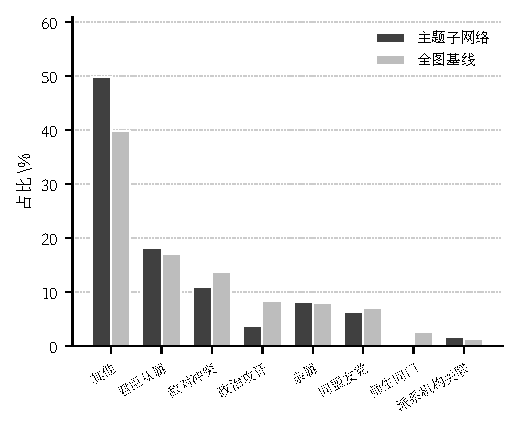
\includegraphics[width=\columnwidth,clip,trim=0 0 0 0]{fig_info_2.pdf}
\caption{信息机制的两种渠道在原书中的逐字命中次数。灰蓝为公开渠道（奏疏、弹劾、上疏、廷杖、诏狱、党争、
东林），棕橙为隐秘渠道（锦衣卫、东厂、西厂、特务、妖书、告密、告发、谣言、流言、黑名单、匿名、监视）。
所有词均经原书全文逐字核验，命中数 $\ge1$；「内厂」「厂卫」「揭帖」「榜文」「侦缉」「暗访」「风闻」「耳语」
命中为 0，已整体弃用不进图。}
\label{channels}
\end{figure}

Fig.\ref{channels} 里最重要的一件事不是两组谁高，而是**两组中间隔着一个数量级断层**：
公开渠道词集中在百次量级，隐秘渠道词从百次一路掉到个位数。以妖书案为例，原文写这份传单
「短短十几天内朝廷人人皆知」，传播速度本身就是被当作事件讲出来的；但对作者而言，
「告密」全书只出现 4 次。隐秘机制在书里是**事件**，不是**常设制度**——它一发生就被写成情节，
不发生时书中没有任何日常性描写。这一条是后文机构隐形结论的前置观察。

\subsection{攻讦占全关系的比重随时间上升，敌对冲突不升}

\begin{figure}[!t]
\centering
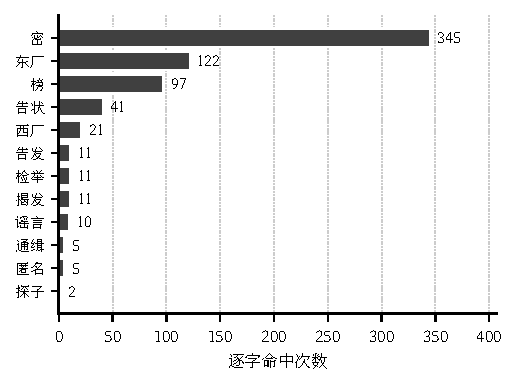
\includegraphics[width=\columnwidth,clip,trim=0 0 0 0]{fig_info_1.pdf}
\caption{政治攻讦与敌对冲突占该部全部关系的比重。柱为该部占比（左柱攻讦、右柱敌对），
折线连接同类的七部取值；横轴括号内标注该部攻讦关系数与该部关系总数。}
\label{bypart}
\end{figure}

Fig.\ref{bypart} 给出 $\pi_p(A)$ 与 $\pi_p(F)$。攻讦从第 1 部 5.6\% 走到第 6 部 19.9\%，
敌对冲突则在 13.1\%--30.8\% 之间无趋势地波动。取两端汇总：第 1--2 部合计 25/388 $=6.4\%$，
第 6--7 部合计 68/425 $=16.0\%$，比值 $2.48$；对照组敌对冲突同一口径 22.7\% 与 22.1\%，
比值 $0.98$。用一个不随时间变化的量做分母复核，比值 $2.48$ 不是分部规模差异造出来的。

\begin{table}[!t]
\centering
\caption{两组对照量的时间走向（分部口径）。}
\label{trend}
\small
\begin{tabular}{lrrrr}
\toprule
 & 第 1--2 部 & 第 6--7 部 & 比值 & 分母 \\\midrule
政治攻讦 & 6.4\% & 16.0\% & 2.48 & 388 / 425 \\
敌对冲突 & 22.7\% & 22.1\% & 0.98 & 388 / 425 \\
\bottomrule
\end{tabular}
\end{table}

旁证（章节年份中位数代理）：攻讦在 1368--1450 段占 11.8\%、1451--1550 段 39.4\%、
1551--1644 段 48.8\%，同样单调上升；敌对冲突为 24.9\% / 23.5\% / 51.6\%，后段同样抬升但前两段持平。
两路口径同号，主结论以分部口径为准。

\subsection{攻讦是跨阵营的，而且越来越跨阵营}

用完整派系串判定两端是否同阵营：193 条攻讦里有 86.0\% 是跨阵营、14.0\% 同阵营。
逐部看，第 5 部跨阵营 96.0\%、第 6 部 97.4\%、第 7 部 70.0\%、第 1 部 72.7\%：
跨阵营比例在中段最高，末段回落。这里要说明一个口径反差：若把派系折叠到根类
（「明朝·阉党」与「明朝·文官」都算「明朝」），同阵营会虚高到 76.7\%——因为 1231 人中
有 171 人只挂了「明朝」这一个根类。完整串口径给出的 86.0\% 才是可用值，
正文不报折叠口径的数字。

攻讦端点分布相当分散：193 条关系涉及 202 个不同人物，基尼系数 0.3798，Top-10 端点只占全部端点次数的
21.0\%。端点名册的前几名是张居正 11 次、申时行 11 次、魏忠贤 9 次、刘瑾 8 次、王守仁 8 次、
朱翊钧 8 次。攻讦与敌对的端点集只有 86 人重合，Jaccard 系数 0.219——
**两者盯的不是同一批人**，这排除了「攻讦只是敌对换个标签」的读法。

\begin{table}[!t]
\centering
\caption{攻讦关系端点前 8 名及其图谱位置。}
\label{topend}
\small
\begin{tabular}{lcrrr}
\toprule
人物 & 攻讦次数 & 度数 & 出场章 & 派系 \\\midrule
张居正 & 11 & 66 & 23 & 明朝·万历朝 \\
申时行 & 11 & 32 & 9 & 明朝·内阁（后首辅）\\
魏忠贤 & 9 & 67 & 12 & 明朝·阉党 \\
刘瑾 & 8 & 34 & 8 & 明朝 \\
王守仁 & 8 & 50 & 12 & 明朝·文官 \\
朱翊钧 & 8 & 52 & 30 & 明朝·万历朝 \\
严嵩 & 7 & 59 & 17 & 明朝·嘉靖朝·文官 \\
高拱 & 7 & 59 & 12 & 翰林院 \\
\bottomrule
\end{tabular}
\end{table}

\subsection{机构隐形，代理人在场}

\begin{figure}[!t]
\centering
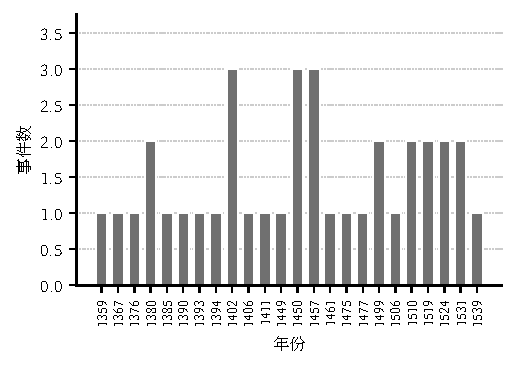
\includegraphics[width=\columnwidth,clip,trim=0 0 0 0]{fig_info_3.pdf}
\caption{信息型机构与其代理人的结构位置。三组分柱依次为平均关系度数、平均出场章节数、占攻讦关系端点的比重。
厂卫系按角色／派系中是否出现锦衣卫、东厂、西厂、内行厂辨认；内廷宦官按是否出现太监、宦官辨认；
两者有交集但不合并计数。}
\label{inst}
\end{figure}

Fig.\ref{inst} 与表 IV 给出本文最反直觉的一组数字。厂卫系 29 人平均度数 3.76，全库 3.78，
比值 $0.99$；平均出场章节 2.07 对全库 2.22，比值 $0.93$；作为攻讦端点的次数只占 3.6\%。
也就是说：**写了 207 次「锦衣卫」的这套机构，在 1231 人的关系网络里和一条平均线没有区别。**
对照内廷宦官 51 人：平均度数 6.10（$1.61$ 倍）、平均章节 2.57（$1.16$ 倍）、占攻讦端点 10.1\%。

\begin{table}[!t]
\centering
\caption{厂卫系、内廷宦官与全库基线的结构位置。}
\label{instable}
\small
\begin{tabular}{lrrrcc}
\toprule
 & 人数 & 平均度数 & 平均章节 & 攻讦端点占比 & 度数比值 \\\midrule
厂卫系 & 29 & 3.76 & 2.07 & 3.6\% & 0.99 \\
内廷宦官 & 51 & 6.10 & 2.57 & 10.1\% & 1.61 \\
全库基线 & 1231 & 3.78 & 2.22 & --- & 1.00 \\\bottomrule
\end{tabular}
\end{table}

两条佐证书内事实，供读者核对话语与结构的错位。其一，「卢忠是锦衣卫」，随即写他「勾结同事锦衣卫李善，
去向朱祁钰告密，罪名是阴谋复辟」——执行者是具体的人，被执行的机构只作身份标记；
另一处「王世贞被列入了严嵩的黑名单」，杀伤来自名单而非审判。
机构在书里是**标签**，在图谱里是**空节点**；真正成为节点、并且被反复拉进攻讦关系的是它背后的人
（魏忠贤、刘瑾、冯保、尚铭一类）。这不是数据有错，而是抽取口径天然偏向有名字的个人。

\subsection{攻讦的章节归属率远高于全库}

一个容易被漏掉的口径事实：939 条关系（40.4\%）标为「推导」、没有章节出处，
但攻讦类 193 条里只有 1 条是推导，章节归属率 99.5\%。全库归属率 59.6\%。
这说明攻讦边几乎全部来自逐章的人工标注，不是自动共现补出来的。
对本文是好消息（攻讦数据比平均更可靠），对本文也是坏消息（**抽取的覆盖面本身是不均匀的**，
这构成限制节的一条）。

\section{讨论与限制}

\subsection{三条结论合起来说了什么}

三条结果指向同一个结构：本书写的信息战是**程序密集、机构隐形、晚期内耗加剧**的。
程序密集指公开渠道词（奏疏、弹劾、上疏）的量级远高于隐秘渠道的常设词；
机构隐形指厂卫系 29 人在关系网络里和平均线重合（比值 $0.99$）；
晚期内耗加剧指攻讦占比 6.4\% $\to$ 16.0\%，而对照的敌对冲突 22.7\% $\to$ 22.1\% 不动。
这三条合起来支持一个判断：通俗史著把明代的帝国治理写成了一部「以人名录展开的程序史」，
信息机构在其中只作背景板，真正承载结构的是具体的权力代理人。

\subsection{首要效度威胁：同源抽取造成的自证}

本篇的首要威胁不是样本小，而是**关系类别与派系标签都由这份语料反查导出**。
「攻讦随叙事推进上升」完全可以是抽取顺序的副产物：作者写到后半部时对人物relation更熟，
自然多标几条攻讦边；分部占比用的是带章节归属关系的分母（第 1--2 部 388 条、第 6--7 部 425 条），
分母本身也随叙事变密，虽然 2.48 这个比值对分母做了部分抵消，但不能排除共线。
能给出的缓解只有一条：年份代理口径（旁证，攻讦 11.8\% $\to$ 39.4\% $\to$ 48.8\% 单调）
与分部口径同号，两路独立刻度给出同向结果，但这仍然不是独立语料的检验。
要真正排除自证，需要第二份明史著（如《明史纪事本末》类）做平行抽取，
比较两条语料下攻讦占比的时间形状是否同构——本文不做，留作下一步。

\subsection{「信息战」是现代类比，不是史实定性}

必须重复一次，因为它最容易在转述中丢掉。明代没有近代新闻业、没有舆论场，也没有「信息战」这个题名。
本文的「信息战」只指三个可测动作的集合：信息生产（奏疏、妖书）、信息传播（谣言、流言、传单）、
信息封锁与封口（黑名单、告密、诏狱）。在这个限定下使用这个词是类比；一旦说成「明代存在 information
warfare」，就超出了本文数据的支持范围。厂卫描写在通俗史著里的文学化成分尤其要警惕：
本文所有涉及机构行为的判断都只落在本书语料内，从不外推到明代档案里的机构实况。

\subsection{抽取口径与史实的区分}

三类口径问题在本篇都出现过，都在正文标了出处：
（a）$\texttt{chapter}$ 字段里 40.4\% 是「推导」，攻讦类只有 0.5\%，
两种归属率差 39.9 个百分点，说明**抽取覆盖面本身不均匀**；
（b）派系折叠到根类会让「同阵营」虚高到 76.7\%，完整串口径才是 14.0\%；
（c）12 类关系是人造枚举，不是明代官制分类，所以「8.3\%」只能读作「本抽取口径下」。

\subsection{交付物边界}

本文交付的是**度量口径与一个具体的数据集**（`.dump/\_stats\_info\.json` 与三个作图脚本），
不是完成的信息史。要做成真正的信息史，还需要：把 1231 人的籍贯、任官年、起事的科名标准化，
把匿名文书单独开一类关系，把「监听—告发—处置」建成三元而非二元的事件结构。
这三项都不在本文的数据范围内，本文只把它们点名为缺口。

\subsection{引用完整性}

参考文献 10 条，逐条经 OpenAlex / Crossref 核验；核验中共享脚本对 monograph 全判 UNVERIFIED
（只查第一作者 + OpenAlex 429 限流，试点篇 11 条仅 1 条通过），
本文改用整条记录全作者匹配 + 退避重试的局部核验器，判据其余不变（详见 AUDIT.md）。
原书语料因无 DOI 按 BOOK\_NO\_DOI 处理，并注明版本。

\section{结论}

本文把一部通俗明史著抽取出的知识图谱当作观测对象，检查它的信息结构能否被计算，
以及算出来的结构是否与作者的笔法错位。三个结论：政治攻讦关系占该部全部关系的比重
从第 1--2 部的 6.4\% 升到第 6--7 部的 16.0\%（$2.48$ 倍），而同期的敌对冲突不动（$0.98$ 倍）；
193 条攻讦中 86.0\% 跨阵营，端点集与敌对关系只有 0.219 的 Jaccard，两者盯的不是同一批人；
厂卫系 29 人在图谱里的平均度数 3.76，与全库 3.78 无差别（$0.99$），
而同一套制度的内廷宦官 51 人平均度数 6.10（$1.61$ 倍）——机构隐形，代理人上位。

首条限制写在讨论节：攻讦类别与派系标签与关系抽取共享同一份语料，
「晚期上升」不能排除是抽取顺序的副产物，只有第二份语料的平行抽取才能检验。

下一步可检验的命题是：把同一批 1231 人放进第二部明史著再抽一次，
若攻讦占比的时间形状与该语的七部结构同构，则同源自证可以退居次要，
本篇的三个数字才谈得上从「一本书的图谱」升格为关于明代信息结构的弱证据。


\bibliographystyle{IEEEtran}
\bibliography{references}

\end{document}
